\documentclass{edpsci}
\usepackage{amsmath,amssymb,graphicx,booktabs,microtype}
\usepackage{etoolbox,balance}
\usepackage[numbers,sort&compress]{natbib}
\usepackage{hyperref}
\usepackage{url}
\urlstyle{rm}
\graphicspath{{figures/}}
\hypersetup{colorlinks=true,citecolor=blue,urlcolor=blue,linkcolor=blue}
\journalname{Acta Acustica}
\renewcommand{\submittedto}{Template preview for}
\articletype{Research article -- preprint}
\hypersetup{pdftitle={Effects of arrival timing, source startup and room reflections on three-microphone sound localization},pdfauthor={Aneesh Arnav Chikkala},pdfsubject={Acta Acustica template preview; unreviewed preprint; not submitted}}
% Keep the supplied class intact; accommodate its header and one unaffiliated author.
\makeatletter
\patchcmd{\@maketitle}{\vbox to 22.7mm}{\vbox to 27mm}{}{\errmessage{EDP title-box patch failed}}
\patchcmd{\makeheadbox}{\vbox to0pt}{\vbox}{}{\errmessage{EDP article-band patch failed}}
\renewcommand{\institutename}{\par\begingroup\parindent=0pt\noindent\@institute\par\endgroup}
\makeatother
% The class uses \doi for article metadata; bibliography entries need a printed DOI.
\renewcommand{\doi}[1]{doi: \href{https://doi.org/#1}{\nolinkurl{#1}}}

\begin{document}
\title{Effects of arrival timing, source startup and room reflections on three-microphone sound localization}
\titlerunning{Arrival timing and source startup in sound localization}
\author{Aneesh Arnav Chikkala}
\authorrunning{Aneesh Arnav Chikkala}
\institute{No institutional affiliation}
\date{8 September 2026. Preprint for author review; not peer reviewed.}
\abstract{Sound localization with a small microphone array depends on how accurately the arrival times of sound are represented. Room reflections and the choice of when to begin recording can also change the result. This paper examines these effects using three microphones and a fixed GCC-PHAT direction estimator. Independent calculations check the direct sound paths and the simulated room responses before a study of 276,480 frame estimates. Matched recordings separate arrival rounding, source startup and reflections, while independent recordings test averaging. At 10 dB signal-to-noise ratio, rounding arrivals increases direct-path root mean square error from $0.923^\circ$ to $2.300^\circ$. In the subset with stronger reverberation, first-frame error is $4.16^\circ$ just after startup, compared with $42.51^\circ$ when the source has already been running. Averaging 128 frames reduces error, but the low and high subsets still differ: $0.835^\circ$ and $10.158^\circ$, respectively. The results show why arrival timing and source history need to be checked before interpreting localization accuracy. A timing-error bound provides an additional check for the array geometry. The findings apply to the stated simulation and do not establish hardware performance or a universal reverberation limit.}
\keywords{Sound localization, microphone arrays, GCC-PHAT, room simulation, arrival timing, source startup}
\maketitle
\raggedbottom

\section{Introduction}
Accurate sound localization with a small microphone array is difficult because the microphones receive the same sound only a short time apart. The system must measure these small time differences and convert them into a direction. Noise can disturb the measurements, while reflections from the room can produce additional arrivals that compete with the direct sound. For a compact system, the microphone spacing and the processing method therefore need to be considered together.

Simulation provides a useful way to study these effects before testing a device. The microphone positions, sound source and room can be controlled, and the same input can be used in several comparisons. However, the simulated signals also depend on choices made in the software. A sound path may arrive between two sample times. Rounding that arrival to the nearest sample changes the signal. Starting the source immediately before each short recording creates another difference: the reflected sound may still be building up when the direction is estimated.

These choices matter for small arrays. At a sampling rate of 48 kHz, consecutive samples are $20.83\,\mu$s apart. Sound travels about 7.15 mm in that time at 343 m/s. The microphone spacing used here is 86.6 mm, so even one sample is a noticeable part of the travel time across the array. A simulation needs to represent arrivals between samples accurately enough for the angular differences being studied.

Generalized cross-correlation is an established method for estimating time delay \citep{knapp}, and GCC-PHAT has already been used with equilateral three-microphone arrays \citep{catur}. Fractional-delay filtering provides established ways to represent arrivals between samples \citep{laakso}. The image-source method models room reflections by replacing reflected paths with paths from mirrored sources \citep{allen}. These methods form the basis of the present work. The contribution is a controlled study of how their implementation and the recording procedure affect the reported accuracy.

The study asks three practical questions. How much does rounding the arrival times change the estimated direction? How different is a recording made just after source startup from one made while the source is already running? How much does averaging several direction estimates help when it is tested on new recordings? Numerical checks are included before these results are interpreted. This follows the distinction between checking a computational implementation and testing whether its physical assumptions describe a real experiment \citep{ernoult}.

The evaluation uses one stationary synthetic source, three ideal matched microphones and three rectangular rooms. It estimates horizontal direction, or azimuth. The purpose is to understand this defined simulation in enough detail that its results can be inspected and repeated. Microphone calibration, device timing and measured-room performance require separate experiments.

\section{Simulation design and implementation}
\subsection{Microphone array and direction estimate}
The microphones form an equilateral triangle in a horizontal plane. Each microphone is 5 cm from the array center, giving 8.66 cm between microphones. The source is placed 1.5 m from the center at the same height. Figure~\ref{fig:geometry} shows the geometry and the comparisons used in the study.

Relative to the array center, the microphone coordinates are
\begin{equation}
\mathbf m_i=R[\cos\phi_i,\sin\phi_i]^T,\qquad
\phi_i\in\{90^\circ,210^\circ,330^\circ\},
\end{equation}
where $R=0.05$ m. The speed of sound is fixed at $c=343$ m/s. For source position $\mathbf s$, the direct sound reaches microphone $i$ at
\begin{equation}
t_i=\frac{\|\mathbf s-\mathbf m_i\|}{c}.
\end{equation}
The difference for a microphone pair is $\tau_{ij}=t_i-t_j$, with $i<j$. There are three pairs, but they share microphones. Their timing errors therefore cannot generally be treated as independent.

The direction estimator uses a plane-wave approximation. For a unit vector $\mathbf u$ pointing toward the source, the ideal pair delays satisfy $A\mathbf u=-c\boldsymbol\tau$, where each row of $A$ is $(\mathbf m_i-\mathbf m_j)^T$. The measured delays are converted to direction through
\begin{equation}
\widetilde{\mathbf u}=-cA^+\widehat{\boldsymbol\tau},\qquad
\widehat\theta=\operatorname{atan2}(\widetilde u_y,\widetilde u_x).
\label{eq:solve}
\end{equation}
Here $A^+$ is the pseudoinverse, which gives a least-squares fit with equal weight for all three pairs. The angle is taken directly from the fitted vector; its length is not forced to one. The actual direct paths come from a source at finite distance, so their wavefront is curved. Even exact arrival times can therefore produce a small error when interpreted by this plane-wave model. The direct-path checks measure this effect separately.

\begin{figure*}[t]
\centering
\includegraphics[width=\textwidth]{fig1_geometry_controls.pdf}
\caption{Microphone arrangement and matched comparisons. The triangle is drawn to scale; the arrow shows source direction only. The source is 1.5 m from the center. Each combination uses the same underlying source and microphone-noise samples for a given recording. ``Onset'' means one source startup at the beginning of the recording.}
\label{fig:geometry}
\end{figure*}

\subsection{Room model and arrival timing}
Each room is a three-dimensional rectangular enclosure. Reflections are specular, meaning that the reflection angle equals the incidence angle. The six walls have pressure-reflection coefficients that do not change with frequency. The model includes spreading loss but excludes diffraction, diffuse scattering, air attenuation and microphone directivity.

For a room side of length $L_a$ and source coordinate $s_a$, the image-source coordinate is
\begin{equation}
s_a^{\mathrm{img}}=2n_aL_a+(1-2p_a)s_a,
\end{equation}
where $n_a\in[-K,K]$ and $p_a\in\{0,1\}$. The numbers of reflections at the low and high walls are $|n_a-p_a|$ and $|n_a|$. A path of length $r$ arrives after $r/c$ seconds and has pressure gain
\begin{equation}
g(r)=\frac{1}{4\pi r}\prod_w\beta_w^{N_w},
\end{equation}
where $\beta_w$ is the pressure-reflection coefficient of wall $w$ and $N_w$ is its reflection count. The final model uses image extent $K=76$ and includes paths up to 1.2 s long. Both limits are checked by extending them further.

For uniform walls, absorption is set using $\alpha=0.161V/(S T_{\mathrm{nom}})$ and $\beta=\sqrt{1-\alpha}$, where $V$ is room volume and $S$ is surface area. The value $T_{\mathrm{nom}}$ is a nominal reverberation setting used to choose absorption. It is not assumed to equal the decay time of the resulting response. The relationship between wall absorption and room decay needs its own checks \citep{bellows}.

Two versions of arrival timing are compared. The fractional version places each arrival on a time grid 32 times finer than the acquisition grid, using linear deposition. A normalized Kaiser-windowed sinc filter then converts the response to the acquisition rate. Its shape parameter is 8.6 and its half-width is 32 acquisition samples. The rounded version places the path directly at sample $\operatorname{round}(f_s r/c)$. Path gains and reflection coverage remain the same, so the comparison isolates the arrival construction. Reflections can also be switched off while retaining the same direct path and response length.

\subsection{Source signal and recording procedure}
The source is a Gaussian random sequence restricted to 300--3400 Hz with a Fourier-domain mask and normalized in root mean square amplitude. The sampling rate is 48 kHz. Every continuous record includes 59,682 source samples before the analyzed interval. This earlier signal allows the room response and acquisition filter to settle before analysis begins.

All three microphone signals pass through the same causal Butterworth bandpass filter at 300--3400 Hz. The SciPy prototype order is four, which produces four second-order sections and a total bandpass order of eight. Independent Gaussian microphone-noise sequences pass through the same filter.

Noise level is defined relative to the steady direct-only signal after filtering, averaged over the microphones and the analysis interval. The stated signal-to-noise ratio (SNR) is this direct-signal power divided by acquired noise power. The same noise samples and scaling are retained when reflections are added. As a result, the stated SNR is not the ratio of total reverberant signal power to noise power.

The source-history comparison uses two recordings. In the steady recording, the source has already been running before analysis begins. In the onset recording, the earlier source samples are set to zero once, while the samples inside the analyzed interval remain identical. The microphone noise is also identical. This represents a single startup, including its transient spectrum, followed by continuous operation.

Each short recording is divided into 32 consecutive, nonoverlapping frames of 2048 samples. A frame lasts 42.667 ms and the full short record lasts 1.365 s. A separate exploratory check restarts the source and acquisition history before every frame. That procedure is reported separately because it repeatedly observes startup instead of a continuous recording.

\subsection{Delay estimation using GCC-PHAT}
GCC-PHAT estimates the relative delay between each microphone pair by finding a peak in a normalized cross-correlation. PHAT refers to phase-transform weighting: the normalization reduces the influence of spectral magnitude. The precise processing steps are fixed throughout this study.

The mean is removed from each frame and a symmetric Hann window is applied. A 4096-point Fourier transform is then used. For microphone spectra $X_i[k]$ and $X_j[k]$, define
\begin{equation}
G_{ij}[k]=X_i[k]X_j^*[k].
\end{equation}
The cross spectrum is normalized using
\begin{align}
d_{ij}[k]&=\max\bigl(|G_{ij}[k]|,q_{ij}\bigr),\\
q_{ij}&=10^{-3}\max_l|G_{ij}[l]|+10^{-12},\\
W_{ij}[k]&=G_{ij}[k]/d_{ij}[k].
\end{align}
The maximum used for $q_{ij}$ is calculated over all bins. Values of $W_{ij}$ outside 300--3400 Hz are then set to zero. This small denominator floor prevents division by nearly zero values.

The inverse transform is evaluated with eightfold correlation sampling. Only delays physically possible for the pair, within $\|\mathbf m_i-\mathbf m_j\|/c$, are searched. A quadratic fit to the peak and its two neighbors refines the delay. The adjustment is limited to one correlation-grid step and then clipped to the physical delay bound. Equation~\ref{eq:solve} converts the resulting three delays into azimuth.

\subsection{Measuring the simulated room response}
Decay is measured from the reverse-integrated squared impulse response, following Schroeder's energy-decay method \citep{schroeder}. Energy is first summed across microphones. The decay slope between $-5$ and $-25$ dB is fitted and extrapolated to 60 dB to obtain T20. Fit quality, early decay time and T30 are also retained.

The direct-to-reverberant ratio (DRR) compares the energies of separately filtered direct and reflected responses. Their interference cross term is saved as well, because direct and reflected energy need not add independently. Each scene also records the arrival times and gains of the direct path and the six first-order reflections. These measurements describe what the simulated room actually produces, beyond its nominal setting.

\section{Quality control and evaluation}
\subsection{Independent numerical checks}
The first checks test the calculation without room reflections. An independent scalar implementation solves the two-by-two normal equations without importing the main direction solver. It checks plane waves, spherical arrivals, cardinal directions and all six microphone-channel permutations. The analytical study covers 720 angles, radii of 0.025, 0.05 and 0.10 m, source distances of 0.5, 1.5, 5 and 20 m, and sampling rates of 16, 48, 96 and 192 kHz: 34,560 conditions in total.

A separate waveform reference evaluates continuous-time harmonic signals directly and compares them with the fractional-delay filter output. Physical bandwidth, recording duration and observation time are matched. This tests signal construction separately from the algebra used to convert delays into direction.

The room check uses another image enumeration and evaluates each path through its exact frequency-domain phase. It does not share the main path generator or its interpolation filter. Path counts, spectra and direction estimates are compared, including cases with unequal walls. Image extent is increased until two successive changes are below $0.05^\circ$ in direction, 1\% in T20 and 0.1\% in the probe spectrum. Response duration and interpolation are also refined, followed by a joint increase of duration and image extent.

The $0.05^\circ$ target is a numerical resolution target for interpreting effects of about $0.5^\circ$ or larger. It is not a required accuracy for an acoustic device. Checks on random recordings are needed as well: a small change in the response can cause a peak-based estimator to choose a different peak. The pilot and main study use separate, repeatable random-input identities.

\subsection{Test conditions and matched comparisons}
The rooms measure $6\times5\times3$, $5\times4\times2.8$ and $8\times6\times3.2$ m. The array is placed at coordinate fractions $(0.5,0.5,0.5)$ and $(0.6,0.45,0.5)$ of each room. Nominal reverberation settings are 0.15, 0.30 and 0.60 s. Twelve source directions are used, at $7.37^\circ+30^\circ j$ for $j=0,\ldots,11$. The minimum source or microphone distance from a wall is 0.312 m.

The main study uses all 216 combinations of room, placement, nominal setting and direction. Each scene is tested at 0, 10 and 20 dB SNR with five independent short recordings. The allocation and analysis rules were fixed before generating the final results (Table~\ref{tab:protocol}).

\begin{table}[t]
\caption{Main evaluation counts. Each frame contains 2048 samples. Pilot, reference and sensitivity checks are additional.}
\label{tab:protocol}\centering\small
\begin{tabular}{@{}lrr@{}}\toprule
Study & Scenes & Estimates\\\midrule
Main room study & 216 & 103,680\\
Seven additional matched variants & 72 & 80,640\\
Long recordings & 72 & 92,160\\\midrule
Total & & 276,480\\\bottomrule
\end{tabular}
\end{table}

Matched comparisons use the centered, nominal-0.15-s state and the offset, nominal-0.60-s state in each room. With 12 directions, this gives 72 scenes. These are called the low and high subsets. Both absorption and placement differ between them; a low-to-high comparison therefore does not isolate reverberation time alone.

At 10 dB, the same five recordings are used for all eight combinations of fractional or rounded arrivals, steady or onset history, and direct or reflected propagation. The fractional/steady/reflected result is reused from the main study only when its inputs match exactly. Five new 128-frame recordings per scene are then used to describe bias and frame dependence, and five different recordings test averaging. These long recordings are separate from both the pilot and the short-record study.

\subsection{Additional geometry and method checks}
A fixed subset of 24 scenes, four directions in each of the six room states, tests a $17^\circ$ array rotation, an unequal triangle, unequal wall absorption and a narrower 300--1700 Hz source band. The acquisition filter and estimator still use 300--3400 Hz in the narrower-band test. Each variation uses five new 32-frame recordings at 10 dB. These checks show how performance changes beyond the main setup; their differences from the base case are not matched causal estimates because the random records also change.

Steered-response power with PHAT weighting (SRP-PHAT) provides a second localization method \citep{dibiase}. It uses the same base recordings, window, band and normalization. Instead of selecting a separate delay peak for each pair, it combines the pair cross spectra at the continuous plane-wave delays predicted for each candidate angle. The angular grid is $0.25^\circ$, with quadratic refinement, and is checked against a $0.05^\circ$ grid. This is a comparison on the stated subset, rather than a general ranking of methods.

\subsection{Error measures and uncertainty}
Angular error is wrapped to $[-180^\circ,180^\circ)$ so that a small crossing of the angle boundary is treated correctly. Root mean square error (RMSE) gives greater weight to large errors. Median absolute error, the 90th percentile, circular bias and the proportion of errors above $5^\circ$ are also recorded. The $5^\circ$ threshold was chosen in advance as a descriptive measure; it is not a hearing or device-acceptance standard.

Uncertainty is estimated with 2000 bootstrap draws \citep{efron}. Each draw selects whole recordings with replacement within each scene. The same selected recordings are used across matched variants. Keeping frames from a recording together avoids treating them as independent experiments. These intervals describe variation from source and noise for the selected scenes. They do not describe uncertainty over all possible rooms.

The matched effects are calculated from signed errors and squared errors. Mean squared error is averaged first; RMSE is its square root. Subtracting two RMSE values does not create an independent error component. Interactions are calculated as differences between matched effects under different conditions. For example, a rounding-by-reflection interaction asks whether the effect of rounding changes when reflections are present. Full per-scene results are retained alongside pooled summaries.

\subsection{Testing averaging on new recordings}
Direction estimates are averaged over blocks of 1, 2, 4, 8, 16, 32, 64 and 128 consecutive frames. Circular averaging is used: directions are averaged as unit vectors before their angle is taken. This avoids errors at the $-180^\circ/180^\circ$ boundary. The longest block lasts 5.461 s.

For small angular errors, the expected mean squared error of an average can be approximated by
\begin{equation}
\operatorname{MSE}(\overline e_n)\simeq b^2+
\frac{1}{n}\left[\gamma_0+2\sum_{\ell=1}^{n-1}
\left(1-\frac{\ell}{n}\right)\gamma_\ell\right].
\label{eq:variance}
\end{equation}
Here $b$ is the persistent mean error, $\gamma_0$ is frame-error variance and $\gamma_\ell$ describes dependence between errors $\ell$ frames apart. The equation separates a mean offset from fluctuations that averaging may reduce.

These quantities are estimated from the five training recordings, with each record centered before estimating covariance. Covariances above lag 32 are omitted; retained nonzero lags receive weights $1-\ell/33$. Negative predicted variances are clipped to zero. A simpler comparison assumes independent frames by setting nonzero-lag covariances to zero.

The approximation is interpreted only where the training estimates are sufficiently concentrated: circular resultant at least 0.95 and absolute circular mean error at most $15^\circ$. This rule was fixed in advance and uses no test recordings. All scenes remain in the measured test results, including those that fail the rule. The rule does not guarantee that rare large errors are absent.

\section{Results}
\subsection{Numerical checks and the corrected room model}
The direct checks agree closely. Plane-wave recovery differs by at most $5.7\times10^{-14}$ degrees, and the independent scalar solver differs by at most $7.3\times10^{-12}$ degrees. The largest difference between the continuous-time waveform reference and the selected fractional-delay filter is $3.7\times10^{-5}$ degrees. Increasing correlation sampling from 8 to 64 changes direct-path estimates by no more than $0.000495^\circ$.

The final independent room check includes about 5.22 million paths per microphone. Its relative spectral difference is $1.13\times10^{-5}$ and its angular difference is $0.000807^\circ$. Earlier checks with coarse image coverage changed one estimate by more than $100^\circ$, and a coarse fractional grid failed the spectral target. These failures were used to improve the numerical settings and are retained in the verification notes.

One further correction was needed after the initial full run. Extending response duration and image extent together changed ten of 960 checked estimates by more than $0.05^\circ$, with a maximum change of $0.16551^\circ$. The original 0.9-s/extent-48 run was preserved and replaced. The final 1.2-s/extent-76 model, with propagation factor 32, passes a joint extension to 1.5 s/extent 96 with a maximum change of $0.01273^\circ$. The complete study was rerun with the same scientific allocation and analysis rules, using new source and noise identities. All results reported below come from that corrected run.

\begin{table}[t]
\caption{Final numerical checks. Values are the largest changes in estimated angle under each check, not localization errors relative to the source.}
\label{tab:verification}\centering\small
\begin{tabular}{@{}lr@{}}\toprule
Check & Change (deg)\\\midrule
Independent full room reference & 0.000807\\
Longer response and larger image extent & 0.012726\\
Propagation grid 32 to 64 & 0.006965\\
Image extent 76 to 84 & 0.000000\\
GCC factor 8 to 16 & 0.025930\\
SRP angular grid refinement & 0.002310\\\bottomrule
\end{tabular}
\end{table}

Table~\ref{tab:verification} and Figure~\ref{fig:numerics} summarize the final checks. On the fixed 24-scene subset, doubling propagation resolution changes estimates by at most $0.006965^\circ$, increasing image extent gives no change, and increasing GCC correlation sampling changes them by at most $0.02593^\circ$. SRP grid refinement changes estimates by at most $0.002311^\circ$. All checked changes are below the $0.05^\circ$ target. This establishes resolution for the tested cases; it is not a worst-case guarantee for every possible input.

\begin{figure*}[t]
\centering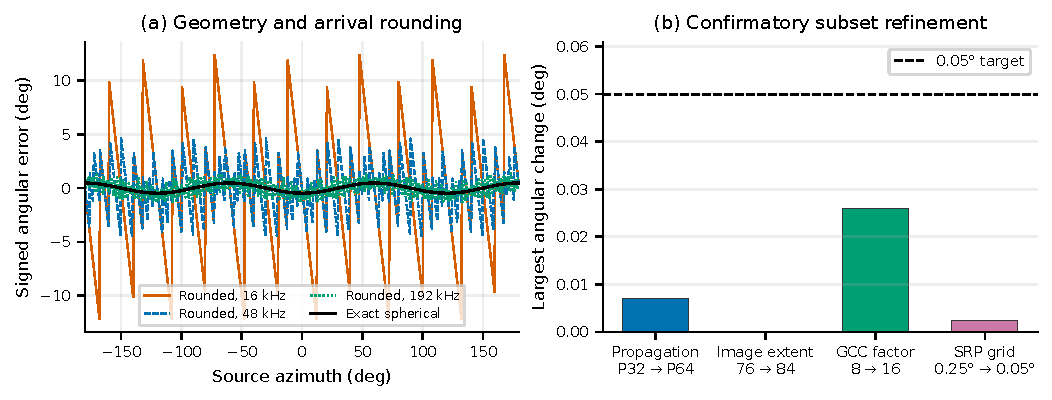
\includegraphics[width=\textwidth]{fig2_numerical_verification.pdf}
\caption{Arrival rounding and numerical resolution. (a) Error from analytical arrival times at radius 0.05 m and source distance 1.5 m. Exact spherical arrivals are processed by the same plane-wave direction solver; these curves do not include waveform noise. (b) Largest changes under refinement on the fixed 24-scene subset, with five recordings and 32 frames per scene. The dashed line marks the $0.05^\circ$ numerical target.}
\label{fig:numerics}
\end{figure*}

The measured T20 ranges are 0.083--0.110 s, 0.259--0.295 s and 0.586--0.683 s for nominal settings of 0.15, 0.30 and 0.60 s. Minimum fit $R^2$ is 0.928 in the lowest setting and 0.994 in the others. Component DRR ranges from about $+9.53$ to $-10.77$ dB. The difference between nominal and measured decay is why the response measurements accompany the room settings.

\subsection{Localization error across rooms}
At 10 dB SNR, RMSE is $1.620^\circ$ for the nominal-0.15-s setting, $11.954^\circ$ for 0.30 s and $37.233^\circ$ for 0.60 s. Their 95\% bootstrap intervals are [1.599, 1.641], [11.168, 12.771] and [36.359, 38.111] degrees. The proportions of estimates with error above $5^\circ$ are 0.86\%, 27.38\% and 62.30\%, respectively.

At 20 dB, RMSE falls to 1.362, 11.796 and $37.067^\circ$. Reducing noise helps, but does not remove the large errors in the more reflective conditions. Figure~\ref{fig:core} shows each room separately so that the pooled trend does not hide room differences.

There is also substantial variation between source directions and array placements. At 10 dB, individual scene RMSE ranges from 0.92 to $3.16^\circ$ in the lowest setting, 2.08 to $49.08^\circ$ in the middle setting and 6.56 to $86.16^\circ$ in the highest. These ranges are much wider than the intervals around the pooled values. A single average therefore cannot describe every scene in the study.

\begin{figure*}[t]
\centering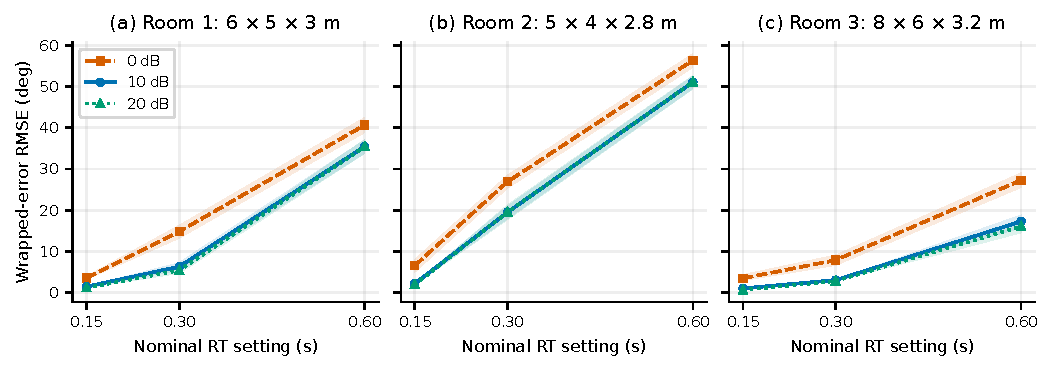
\includegraphics[width=\textwidth]{fig3_core_rooms.pdf}
\caption{Main room results with fractional arrivals and a source already running. Each point combines two array placements, 12 directions and five 32-frame recordings. Shaded bands are 95\% record-bootstrap intervals for those fixed scenes. The horizontal axis gives the nominal setting used to choose wall absorption; actual T20 was measured separately.}
\label{fig:core}
\end{figure*}

\subsection{Effect of rounding arrival times}
Across the 72 matched scenes at 10 dB, steady direct-path RMSE is $0.923^\circ$ [0.912, 0.934] with fractional arrivals and $2.300^\circ$ [2.287, 2.313] with rounded arrivals. The matched increase in mean squared error is 4.438 deg$^2$ [4.380, 4.493]. Thus, the rounding effect remains after waveform generation, filtering and delay estimation; it is not limited to a calculation using exact delays.

With reflections included, steady RMSE is $27.365^\circ$ for fractional arrivals and $28.112^\circ$ after rounding. The matched mean-squared-error increase is 41.448 deg$^2$ [11.974, 70.571]. This does not mean rounding has the same effect in every scene. Reflected paths interfere with one another, and changing their arrival times can change the correlation peak selected by the estimator.

\subsection{Effect of source startup}
The largest difference appears in the first frame after startup. In the high subset, RMSE is $4.157^\circ$ for the newly started source, compared with $42.508^\circ$ when the source has already been running. By the last frame of the 1.365-s recording, both matched conditions reach $41.526^\circ$. Figure~\ref{fig:paired} shows how the early advantage disappears as reflected sound builds up.

This is a change in the observed sound field. The localization algorithm has not improved between the two conditions. A procedure that restarts the source before every short frame can repeatedly measure this easier startup period and report accuracy that does not describe continuous operation. The exploratory frame-reset check shows this behavior as well, but uses pilot directions and is kept separate from the main time trajectory.

For fractional reflected signals across all 72 scenes and 32 frames, startup reduces mean squared error by 42.798 deg$^2$ [22.983, 62.404]. Table~\ref{tab:effects} reports this as onset minus steady, giving a negative difference. The onset-by-reflection interaction is $-49.046$ deg$^2$ [$-65.574$, $-32.891$], while rounding-by-reflection is 30.762 deg$^2$ [4.770, 57.791]. These interactions show that the effects cannot be combined as separate, independent error allowances.

\begin{table}[t]
\caption{Matched changes in mean squared error (deg$^2$) across 72 scenes at 10 dB. Positive values mean more error. Intervals resample whole recordings within each scene.}
\label{tab:effects}\centering\small
\begin{tabular}{@{}lrr@{}}\toprule
Comparison & Change & 95\% interval\\\midrule
Rounding, direct & 4.44 & [4.38, 4.49]\\
Rounding, reflected & 41.45 & [11.97, 70.57]\\
Onset, reflected & -42.80 & [-62.40, -22.98]\\
Reflections, fractional & 747.97 & [699.52, 799.81]\\\bottomrule
\end{tabular}
\end{table}

\begin{figure*}[t]
\centering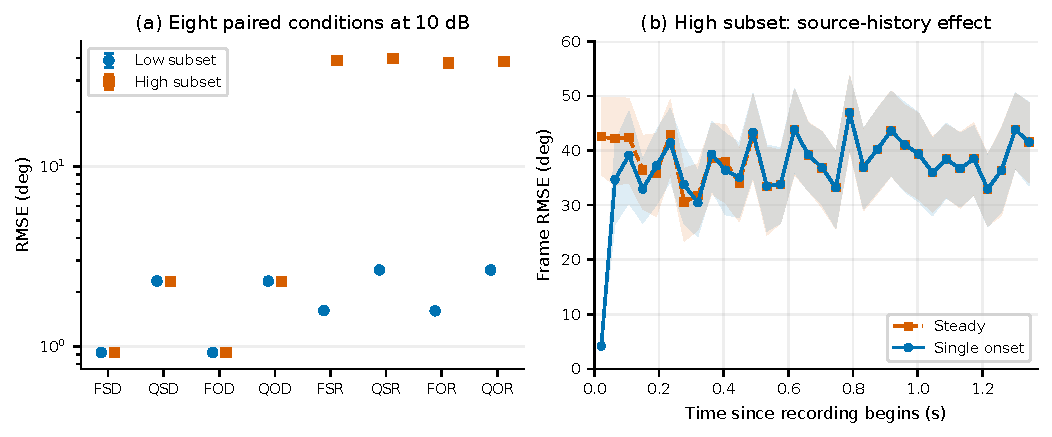
\includegraphics[width=\textwidth]{fig4_paired_attribution.pdf}
\caption{Arrival timing and source startup at 10 dB. (a) All eight combinations: F/Q means fractional/rounded, S/O means steady/onset and D/R means direct/reflected. Low and high subsets contain 36 scenes each and differ in placement and absorption. Error bars resample recordings. (b) Matched fractional reflected recordings in the high subset. The source has already been running in the steady condition. Markers show frame midpoints after analysis begins.}
\label{fig:paired}
\end{figure*}

\subsection{Improvement from averaging}
Averaging reduces error on the independent test recordings (Figure~\ref{fig:averaging}). In the low subset, RMSE falls from $1.597^\circ$ [1.584, 1.610] for one frame to $0.835^\circ$ [0.815, 0.854] for 128 frames. In the high subset, it falls from $39.044^\circ$ [38.439, 39.607] to $10.158^\circ$ [9.404, 10.995]. Even at 128 frames, 46.11\% of high-subset block estimates have error above $5^\circ$.

Forty-nine of the 72 scenes pass the training rule for interpreting the small-error model. Their 128-frame test RMSE is $2.013^\circ$ [1.932, 2.090]. The prediction including frame covariance is $2.075^\circ$, and the independent-frame prediction is $2.106^\circ$. The longer-duration result is close to both predictions on this selected set, while differences at shorter durations remain visible. The small difference between the two predictions does not show a useful advantage from covariance correction here.

All 72 scenes remain in the measured averaging curves. The selected 49-scene analysis is used only to assess the approximation. The remaining errors after 5.46 s depend on the chosen scene and estimator; this finite recording length cannot establish a universal or infinite-time reverberation limit.

\begin{figure*}[t]
\centering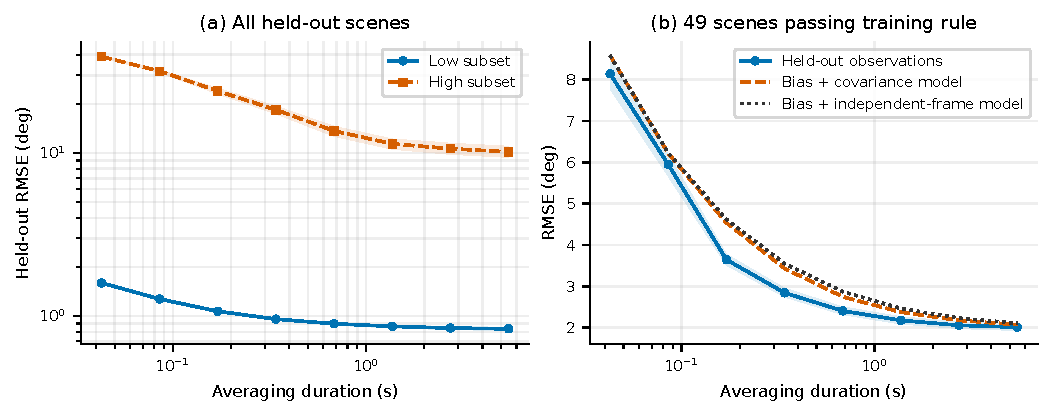
\includegraphics[width=\textwidth]{fig5_heldout_averaging.pdf}
\caption{Averaging tested on new recordings. (a) Circular block averages for all 72 scenes, separated into low and high subsets. (b) The 49 scenes that satisfy the rule set using training recordings. Model curves are predictions, while shaded bands are bootstrap intervals from complete test recordings. Training and test inputs are separate.}
\label{fig:averaging}
\end{figure*}

\subsection{A timing-precision check for the array}
An additional calculation connects microphone-arrival error to direction error. Let $B$ form pair differences from the three microphone arrivals, and let $M$ contain the microphone coordinates, so $A=BM$. If the arrival errors are $\boldsymbol\epsilon$, the change in the fitted direction vector is exactly
\begin{equation}
\delta\widetilde{\mathbf u}=J\boldsymbol\epsilon,\qquad J=-cA^+B.
\end{equation}
This keeps the dependence caused by microphones appearing in more than one pair.

Suppose each arrival error is bounded by $h$. Evaluating the eight combinations $\epsilon_i=\pm h$ gives $\rho=\max\|J\boldsymbol\epsilon\|$. If $\rho<\|\widetilde{\mathbf u}\|$, the largest angular change occurs at a corner of the transformed error box. A simpler conservative bound is
\begin{equation}
|\delta\theta|\leq\arcsin\frac{\rho}{\|\widetilde{\mathbf u}\|}.
\label{eq:bound}
\end{equation}
For the centered equilateral array and a plane wave, $\rho=4ch/(3R)$ and $\|\widetilde{\mathbf u}\|=1$. To keep this change below $\eta$, it is sufficient that
\begin{equation}
h\leq\frac{3R}{4c}\sin\eta.
\end{equation}
At $R=0.05$ m and $\eta=0.5^\circ$, the permitted absolute error per arrival is at most $0.954\,\mu$s. This is a check on ideal arrival times interpreted by the direction solver. It is not a necessary sampling-rate requirement or a guarantee for noisy GCC-PHAT estimates.

All 34,560 rounded-arrival cases satisfy the exact corner bound. Another 12,000 random perturbations, including unequal triangles and an independent scalar solve, give no violations. Figure~\ref{fig:precision}(a) measures change from the exact spherical-arrival estimate. Error between that estimate and the true source direction remains a separate finite-distance effect.

\subsection{Other geometries and the SRP-PHAT comparison}
On the 24-scene subset, GCC-PHAT RMSE is $22.413^\circ$ in the base case. It is $23.729^\circ$ after rotation, $19.644^\circ$ for the unequal triangle, $23.643^\circ$ with unequal walls and $42.054^\circ$ for the narrower-band source (Figure~\ref{fig:precision}(b)). These are limited checks with new random records. They do not establish an optimized geometry. In the narrower-band case, part of the fixed estimator band contains noise without useful source energy.

On the same base recordings, SRP-PHAT gives $30.262^\circ$ RMSE compared with $22.413^\circ$ for GCC-PHAT. However, its proportion of errors above $5^\circ$ is lower: 28.62\% versus 30.57\%. The matched SRP-minus-GCC mean-squared-error difference is 413.473 deg$^2$ [268.788, 561.435]. The disagreement between the two measures shows why the error distribution matters: fewer threshold crossings can coexist with a larger penalty from large errors. Neither measure supports a general method ranking from this subset alone.

\begin{figure*}[t]
\centering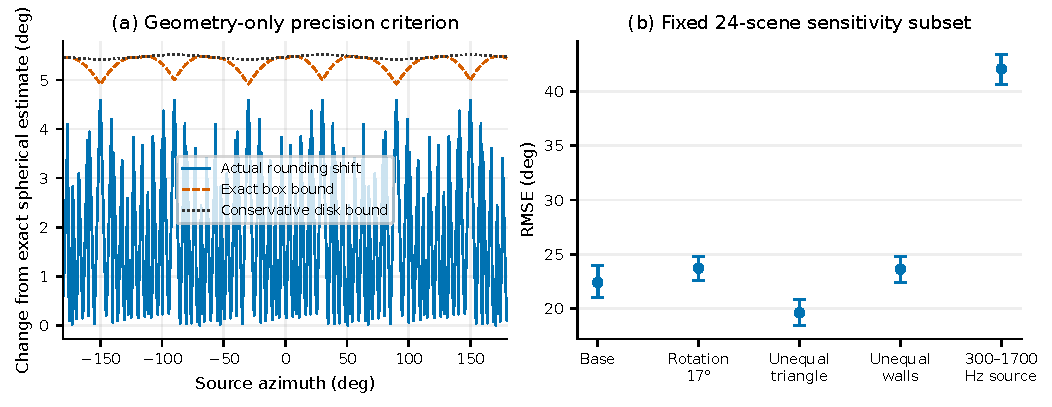
\includegraphics[width=\textwidth]{fig6_precision_sensitivity.pdf}
\caption{Timing precision and additional checks. (a) Analytical rounding changes and their bounds at 48 kHz, radius 0.05 m and source distance 1.5 m. Change is measured from the exact spherical-arrival estimate. (b) RMSE and record-bootstrap intervals for five conditions on the fixed 24-scene subset. The narrower source band retains the 300--3400 Hz acquisition and estimator bands.}
\label{fig:precision}
\end{figure*}

\section{Discussion and practical use}
The main lesson is that the way a simulated recording is generated can change the condition being tested. Rounding the arrivals produces a measurable direct-path penalty. Beginning with no earlier source signal can produce a much larger apparent improvement in the first reflected-sound frame. Both effects need to be checked before the reported error is attributed to the array or localization method.

For continuous operation, the simulated source needs enough earlier history for the selected room response and acquisition filter. If startup is the intended application, it should be studied explicitly as startup. Using the same analyzed source samples and noise across conditions makes that distinction testable. Resetting every frame answers a different question from estimating direction continuously in an already active room.

The correction during numerical review also matters. A long response cutoff alone does not ensure that all influential paths are included if the image extent is too small. Conversely, agreement in a spectral norm does not by itself guarantee agreement between the peaks chosen by a direction estimator. Checking both the response and the resulting angles, including a joint extension of duration and image extent, exposed the initial limitation and led to the complete rerun.

Averaging is useful, but its benefit needs to be measured on recordings that were not used to estimate the prediction model. It reduces fluctuations without changing the room geometry, wavefront curvature or a stable preference for an incorrect correlation peak. The present results show different remaining errors in different scenes. They do not establish an error floor determined by reverberation time alone.

Several limits apply when using these findings in a device study. The microphones are ideal and matched, so the simulation excludes gain mismatch, clock drift and calibration error. The source is band-limited Gaussian noise, rather than speech or a machine. The walls are frequency independent and reflect specularly. Real surfaces, scattering and directional microphones can change the sound field. The main study also uses one array size and source distance, although the analytical timing checks cover a wider range.

The bootstrap intervals use five independent short recordings per scene and describe only the selected scenes. Their coverage has not been separately calibrated, and individual-scene intervals have limited resampling support. Three room geometries do not represent all rooms. Complete scene results, difficult estimates and input identities are therefore supplied with the pooled values. A measured-room study would provide the next test of physical transfer; the present work provides numerical verification and a repeatable simulation comparison.

\section{Conclusion}
This study separates arrival rounding, source startup and room reflections in a three-microphone localization simulation. Rounding increases direct-path error after waveform processing. Starting a source immediately before analysis can make the first frame appear much more accurate than a recording made during steady operation. Averaging new recordings reduces error, but leaves different remaining errors across the tested scenes.

Independent calculations and refinement checks establish numerical resolution for the reported comparisons. A geometry-based timing bound provides a further check for ideal arrivals while retaining shared-microphone dependence. Together, the results give a practical basis for checking simulated localization accuracy and reporting the recording conditions that produced it. They do not establish hardware accuracy, universal estimator superiority or a general reverberation-error law.

\funding
This work was self-funded by Aneesh Arnav Chikkala. The author has no institutional affiliation.

\conflict
Author confirmation of the conflict-of-interest declaration is pending for this review version.

\authorcontrib
Aneesh Arnav Chikkala selected the research direction and funded the work. Final scientific review and release approval remain pending. OpenAI Codex assisted with planning, mathematical derivations, implementation, numerical checks, literature synthesis, analysis, figures and manuscript drafting. The figures were generated by deterministic plotting code from retained results. This assistance included substantive research and writing work. The internal computational checks are not external peer review.

\dataavailability
The accompanying source and data package contains per-frame results, configurations, code, figures, environment records and reproduction instructions. A fresh environment reproduced 8,640 representative estimates exactly and all six main PNG figures byte for byte. This was a representative rerun, not another complete revised campaign. No public archive identifier has been assigned. Licenses and public release await the author's decision.

\supplementary
The accompanying supplement gives the extended model, derivations, numerical correction, statistical details and reproduction record. The original run is retained separately for audit; the paper uses only the corrected results.

\bibliographystyle{unsrtnat}
\balance
\begingroup\interlinepenalty=10000
\bibliography{references}
\endgroup
\end{document}
